\documentclass[10pt,letterpaper]{article}

% --- Page layout ---
\usepackage[margin=1in]{geometry}
\usepackage[skip=0.8em]{parskip}
\usepackage{setspace}
\setstretch{1.15}

% --- Fonts (LuaLaTeX): OpenType text + OpenType math ---
\usepackage{unicode-math} % loads fontspec automatically under LuaLaTeX [web:53]
\setmainfont{Libertinus Serif}
\setsansfont{Libertinus Sans}
\setmonofont{Libertinus Mono}
\setmathfont{Libertinus Math}

% --- Typography ---
\usepackage{microtype} % protrusion+expansion work with LuaTeX [web:55]

% --- Math / units ---
\usepackage{amsmath}
\usepackage{siunitx}
\sisetup{separate-uncertainty=true}

% --- Figures / tables ---
\usepackage{graphicx}
\usepackage{float}
\usepackage{caption}
\usepackage{booktabs}
\usepackage[table]{xcolor} % enables row/cell coloring in tables

% --- Section formatting / quotes ---
\usepackage{titlesec}
\usepackage{csquotes}

% --- Links (load late) ---
\usepackage{hyperref} % rule of thumb: load hyperref last [web:54]
\hypersetup{
  colorlinks=true,
  linkcolor=blue,
  filecolor=magenta,
  urlcolor=cyan,
  citecolor=blue,
  pdftitle={Virial Mass Estimation of ACO 2670},
  pdfauthor={Jackson Ferguson},
}

% --- Misc stability ---
\setlength{\emergencystretch}{3em}
\setlength{\columnsep}{20pt}

% Title Information
\title{Estimating the Virial Mass and Mass-to-Light Ratio of a Rich Galaxy Cluster with SDSS-DR18 Data}
\author{
  \textbf{Jackson Ferguson} \\
  University of Victoria \\
  Astrophysics
}

\date{March 2025}

\begin{document}

% Start the two-column mode, but inject a single-column header first
\twocolumn[
  \begin{@twocolumnfalse}
    \maketitle

    \vspace{1em}

    % --- NARROW ABSTRACT FIX ---
    \centering % This centers the minipage box itself
    \begin{minipage}{0.9\textwidth} % Constrain width to 80% of the page
      \begin{abstract}
        \noindent
        We present a virial mass estimation of the galaxy cluster ACO 2670 using photometric and spectroscopic data from SDSS DR18. By analyzing the radial and redshift distributions of 98 confirmed member galaxies, we determine a cluster redshift of $z = 0.0764$ and a velocity dispersion of $\sigma_v = \SI{932 \pm 95}{km s^{-1}}$. We derive a virial mass of $M_{1/2} = (6.45 \pm 1.31) \times 10^{14} M_{\odot}$ and a mass-to-light ratio of $(291 \pm 60) M_{\odot}/L_{\odot}$, confirming the presence of a dominant dark matter halo.
      \end{abstract}
    \end{minipage}
    % ---------------------------

    \vspace{3em} % Increased space slightly to balance the tighter width

  \end{@twocolumnfalse}
]

\section{Introduction}
Galaxy clusters, the most massive gravitationally bound structures in the universe, serve as critical laboratories for studying dark matter, galaxy evolution, and large-scale structure formation \cite{zwicky1933}. Their dynamical properties, such as virial mass and mass-to-light ($M/L$) ratios, provide key insights into the distribution of luminous and dark matter. However, estimating these quantities requires careful analysis of observational data, robust statistical methods, and assumptions that may influence the results. This study focuses on the galaxy cluster ACO 2670, utilizing photometric and spectroscopic data from the Sloan Digital Sky Survey (SDSS) Data Release 18 (DR18) \cite{york2000} to determine its virial mass, luminosity distribution, and $M/L$ ratio. The analysis hinges on several foundational assumptions:

\begin{enumerate}
  \item \textbf{Virial Equilibrium:} The cluster is assumed to be dynamically relaxed, enabling the application of the virial theorem. This assumption may not hold for systems with substructure or ongoing mergers, as suggested by ACO 2670's irregular spatial distribution.
  \item \textbf{Cosmological Model:} Distance calculations rely on the Flat $\Lambda$CDM cosmology, with fixed Hubble constant ($H_{0}$) and matter density ($\Omega_{m}$) values. Uncertainties in these parameters propagate to distance and mass estimates.
  \item \textbf{Data Completeness:} SDSS spectroscopic data are assumed to represent a complete and unbiased sample of cluster galaxies, though selection effects (e.g., fiber collisions, magnitude limits) may exclude faint or crowded objects.
  \item \textbf{Projection Effects:} Galaxy velocities and positions are analyzed in projection, neglecting the three-dimensional structure of the cluster.
  \item \textbf{Iterative Membership Selection:} The \SI{1.5}{Mpc} radial cutoff and $\pm3\sigma$ redshift clipping are assumed to effectively isolate true cluster members, though interlopers or incomplete sampling may persist.
\end{enumerate}

The analysis assumes a Flat $\Lambda$CDM cosmology with parameters from Planck Collaboration et al. \cite{planck2020}: Hubble constant $H_{0}=67.4\,\text{km}\,\text{s}^{-1}\text{Mpc}^{-1}$, matter density $\Omega_{m}=0.315$, and dark energy density $\Omega_{\Lambda}=0.685$. These values define the universe's expansion history and were used for luminosity distance calculations.

This work employs a multi-step methodology: refining cluster membership iteratively, computing the weighted cluster center, analyzing redshift distributions using the Freedman-Diaconis rule \cite{freedman1981} and Bayesian Information Criterion \cite{schwarz1978}, calculating relativistic distances \cite{harrison1993, astropy2022}, and applying the virial theorem to estimate mass. The derived $M/L$ ratio is contextualized against stellar population models to infer dark matter content.

\section{Data Acquisition and Cleaning}
To analyze the ACO 2670 galaxy cluster, photometric and spectroscopic data were retrieved from the Sloan Digital Sky Survey (SDSS) Data Release 18 (DR18). The dataset included the positions, magnitudes, extinction corrections, and redshifts of galaxies in a \SI{2}{Mpc} region centered on the cluster. The SQL query used for data retrieval applied spatial and redshift constraints to ensure that the sample included only galaxies near the cluster while filtering out foreground and background objects. The initial member selection used a $3\sigma$ clipping method, retaining galaxies within three standard deviations of the mean redshift.

During data analysis, an outlier galaxy with an unusually dim absolute magnitude ($M_{r}=-16$) was identified. Inspection of the SDSS Explore tool revealed that this object was photometrically classified as a star and flagged for edge deblending and saturation. Despite its spectroscopic classification as a galaxy, the photometric flags and star-like properties suggested unreliable data. This object was excluded to prevent photometric outliers from biasing the luminosity-weighted centroid.

\section{Spatial Analysis and Centroid Determination}
To analyze the spatial distribution of galaxies in ACO 2670, a scatter plot of Right Ascension (RA) vs. Declination (Dec) was created (Figure \ref{fig:radec_initial}).

\begin{figure}[htb]
  \centering
  \includegraphics[width=0.9\columnwidth]{figures/initial_sky_distribution.pdf}
  \caption{RA-Dec Distribution of Galaxies in ACO 2670.}
  \label{fig:radec_initial}
\end{figure}

The resulting plot revealed a clear concentration of galaxies around the center of the plot, but without a well-defined, sharply bounded core. Instead of a smooth density gradient transitioning from high-density central regions to lower-density outskirts, the galaxy distribution was irregular, with varying densities and possible substructures. The cluster did not exhibit perfect symmetry, and a mild elongation along the positive diagonal (RA increasing with Dec) was observed.

A key challenge in this step was interpreting the structural properties of the cluster. Unlike relaxed clusters with clear, well-defined centers, ACO 2670 showed evidence of substructure, possibly indicating a dynamically active system or recent mergers. These characteristics suggest that ACO 2670 may not be in a fully virialized state, which could impact subsequent mass estimates.

\subsection{Weighted Mean Cluster Center}
We compute the weighted mean Right Ascension (RA) and Declination (Dec) using inverse squared $r$-band magnitude errors as weights. Additionally, we determine the uncertainties associated with these weighted means.

\subsubsection*{1. Compute the Weights}
The weights are based on the inverse squared $r$-band magnitude errors:
\begin{equation}
  w_{i}=\frac{1}{\sigma_{r,i}^{2}}
\end{equation}
where $w_{i}$ is the weight for galaxy $i$ and $\sigma_{r,i}$ is the $r$-band magnitude error for galaxy $i$.

\subsubsection*{2. Compute the Weighted Mean RA and Dec}
The weighted mean Right Ascension ($\overline{\alpha}$) and weighted mean Declination ($\overline{\delta}$) are calculated as:
\begin{equation}
  \overline{\alpha}=\frac{\sum_{i}w_{i}\alpha_{i}}{\sum_{i}w_{i}}, \quad \overline{\delta}=\frac{\sum_{i}w_{i}\delta_{i}}{\sum_{i}w_{i}}
\end{equation}
where $\alpha_{i}$ and $\delta_{i}$ are the RA and Dec of galaxy $i$, and $w_{i}$ is the corresponding weight.

\subsubsection*{3. Compute the Weighted Variance}
The weighted variance accounts for both the measurement errors and the intrinsic scatter in the data. We compute the weighted variances as:
\begin{align}
  \sigma_{\alpha}^{2} &= \frac{\sum_{i}w_{i}(\alpha_{i}-\overline{\alpha})^{2}}{\sum_{i}w_{i}} \cdot \frac{N}{N-1} \\
  \sigma_{\delta}^{2} &= \frac{\sum_{i}w_{i}(\delta_{i}-\overline{\delta})^{2}}{\sum_{i}w_{i}} \cdot \frac{N}{N-1}
\end{align}
where $N$ is the number of member galaxies. The factor $\frac{N}{N-1}$ is a bias correction for the weighted variance to ensure an unbiased estimator.

\subsubsection*{4. Compute the Standard Error of the Weighted Mean}
The uncertainty in the weighted mean RA and Dec is given by:
\begin{equation}
  \sigma_{\overline{\alpha}}=\sqrt{\frac{\sigma_{\alpha}^{2}}{\sum_{i}w_{i}}}, \quad \sigma_{\overline{\delta}}=\sqrt{\frac{\sigma_{\delta}^{2}}{\sum_{i}w_{i}}}
\end{equation}
The final computed cluster center was at $\overline{\alpha}=(358.5546\pm0.0003)^{\circ}$, $\overline{\delta}=(-10.3768\pm0.0003)^{\circ}$. This result provides a more accurate sky position of the galaxy cluster compared to a simple arithmetic mean, as it accounts for measurement uncertainties.

One challenge was ensuring that the weighting method was appropriate, alternative weighting schemes, such as using the r-band magnitudes directly, could have been considered. Additionally, missing or zero-error values in the dataset could have affected the calculations, requiring proper filtering before computing the weighted mean.

Another challenge I had was determining what level of precision to report my results. The computed cluster center (RA, Dec) is reported to four decimal places, as SDSS astrometric uncertainties are typically 0.03–0.3 arcseconds (~0.000008–0.00008 degrees). This level of precision ensures that the reported values are meaningful and not artificially over-precise relative to the data quality.

\section{Kinematics and Velocity Dispersion}
The redshift distribution of the cluster provides crucial insights into its dynamical state and potential substructures. By analyzing the histogram of galaxy redshifts, we can determine the cluster's mean redshift ($z_{cluster}$) and velocity dispersion. A single Gaussian fit is commonly used to describe relaxed clusters, but deviations from a Gaussian distribution can indicate merging substructures. To ensure a robust analysis, we compare a single Gaussian fit to a Gaussian Mixture Model (GMM) with two components, selecting the best model using the Bayesian Information Criterion (BIC).

\subsubsection*{1. Binning the Redshift Data}
The optimal bin width $\Delta z$ is chosen using the Freedman-Diaconis rule:
\begin{equation}
  \Delta z=\frac{2\times \text{IQR}(z)}{N^{1/3}}
\end{equation}
where $\text{IQR}(z)$ is the interquartile range of the redshifts, and $N$ is the number of galaxies. If this bin width is too small, we use Scott's rule as an alternative:
\begin{equation}
  \Delta z=\frac{3.5\sigma_{z}}{N^{1/3}}
\end{equation}
The number of bins is then:
\begin{equation}
  N_{bins}=\frac{z_{max}-z_{min}}{\Delta z}
\end{equation}

\subsubsection*{2. Fitting a Weighted Gaussian to the Redshift Distribution}

The probability density function of a Gaussian is given by:
\begin{equation}
  f(z) = A \exp\left(-\frac{(z-\mu)^{2}}{2\sigma^{2}}\right)
\end{equation}
where $A$ is the amplitude, $\mu$ is the mean redshift $(z_{cluster})$, and $\sigma$ is the standard deviation (redshift dispersion). Since redshift errors $\sigma_{z_{i}}$ vary per galaxy, we use inverse variance weighting:
\begin{equation}
  w_{i} = \frac{1}{\sigma_{z_{i}}^{2}}
\end{equation}
The weighted mean and standard deviation are computed as:
\begin{align}
  \mu_{w} &= \frac{\sum w_{i}z_{i}}{\sum w_{i}} , \quad \sigma_{w} = \sqrt{\frac{\sum w_{i}(z_{i}-\mu_{w})^{2}}{\sum w_{i}}}
\end{align}
These values serve as initial estimates for fitting the Gaussian function to the binned redshift data.

\subsubsection*{3. Gaussian Mixture Model (GMM) and Model Comparison}

The GMM assumes the redshift distribution is a sum of two Gaussian components:
\begin{equation}
  f(z) = \sum_{i=1}^{2} w_{i} \cdot \frac{1}{\sqrt{2\pi\sigma_{i}^{2}}} \exp\left(-\frac{(z-\mu_{i})^{2}}{2\sigma_{i}^{2}}\right)
\end{equation}
where $w_{i}$ are the mixture weights, and $\mu_{i}, \sigma_{i}$ are the means and standard deviations of the components. The Bayesian Information Criterion (BIC) evaluates the model complexity and fit:
\begin{equation}
  \text{BIC} = k \ln(N) - 2 \ln(L)
\end{equation}
where $k$ is the number of parameters and $L$ is the maximum likelihood estimate. A lower BIC indicates a better model. For the single Gaussian, we estimate the log-likelihood as:
\begin{equation}
  \ln(L) = \sum \ln f(z_i)
\end{equation}
and compute its BIC. The GMM BIC is obtained directly from the model fit. If the GMM has a significantly lower BIC and both components have non-negligible weights, we select it as the better model.

\begin{figure}[htb]
  \centering
  \includegraphics[width=0.9\columnwidth]{figures/initial_redshift_distribution.pdf}
  \caption{Redshift Distribution with Optimal Binning and Model Fitting. The single Gaussian model (red) is compared against a GMM (green).}
  \label{fig:redshift_dist}
\end{figure}

The redshift histogram follows a Gaussian distribution, with a clear peak at $0.07642 \pm 0.00346$. The BIC values indicate that the single Gaussian ($\text{BIC} = -871.8$) provides a significantly better fit than the GMM ($\text{BIC} = -840.3$). Additionally, the second GMM component has a negligible weight ($0.03$), confirming that no significant substructure is detected in the redshift space. The use of the GMM was motivated by the possibility of merging substructures, which could be revealed in later steps through spatial and velocity dispersion analysis. However, in this case, the GMM did not improve the fit, suggesting that the cluster is relatively well-virialized in redshift space. The cluster's velocity dispersion derived from the redshift spread will be critical for mass estimation in subsequent steps.

\subsection{Distance Estimation}

The distance to the galaxy cluster ACO 2670 was initially estimated using Hubble's Law. First, the recessional velocity was calculated using the Doppler shift approximation $v_{rec} \approx c z$. While this method is commonly used for rough distance estimates, it does not account for relativistic effects or the expansion history of the universe, which can introduce errors at higher redshifts.

\subsubsection*{1. Recessional Velocity Using the Relativistic Doppler Formula}
To improve accuracy, a relativistic Doppler shift formula was implemented to refine the recessional velocity calculation:
\begin{equation}
  v_{rec} = c \cdot \frac{(1+z)^{2}-1}{(1+z)^{2}+1}
\end{equation}
where $c$ is the speed of light and $z$ is the redshift of the cluster. This correction is important for objects at moderate redshifts ($z \approx 0.08$), where the simple linear approximation begins to deviate from reality. To compute the uncertainty in $v_{rec}$, we propagate the uncertainty in redshift ($\sigma_{z}$):
\begin{equation}
  \frac{dv_{rec}}{dz} = c \cdot \frac{4(1+z)}{[(1+z)^{2}+1]^{2}} \implies \sigma_{v_{rec}} = \left| \frac{dv_{rec}}{dz} \right| \sigma_{z}
\end{equation}

\subsubsection*{2. Luminosity Distance Using Cosmology}
The cluster's luminosity distance is obtained from the Flat $\Lambda$CDM cosmology:
\begin{equation}
  d_{L} = D_{L}(z)
\end{equation}
where $D_{L}(z)$ is the luminosity distance function from the Astropy cosmology model. We approximate the uncertainty in distance due to redshift by computing the numerical derivative:
\begin{equation}
  \frac{dD_{L}}{dz} \approx \frac{D_{L}(z+\delta z)-D_{L}(z-\delta z)}{2\delta z}
\end{equation}
where $\delta z$ is a small redshift step ($\delta z = \sigma_{z}/10$). Thus, the uncertainty due to redshift is:
\begin{equation}
  \sigma_{D_{L},z} = |dD_{L}/dz|\sigma_{z}
\end{equation}
Since the distance scales inversely with the Hubble constant ($H_{0}$), we estimate the uncertainty due to $H_0$ as:
\begin{equation}
  \sigma_{D_{L},H_{0}} = D_{L} \times \frac{\sigma_{H_{0}}}{H_{0}}
\end{equation}
The total uncertainty in distance is combined using quadrature addition:
\begin{equation}
  \sigma_{D_{L}} = \sqrt{\sigma_{D_{L},z}^{2} + \sigma_{D_{L},H_{0}}^{2}}
\end{equation}

I calculated a recessional velocity of $(21962.31 \pm 928.65) \, \text{km}\,\text{s}^{-1}$ and a cluster distance of $(355.87 \pm 16.66) \, \text{Mpc}$.

\subsection{Projected Radial Distribution}

To analyze the spatial distribution of the cluster members, I implemented a function to compute the projected distances of galaxies from the cluster center in megaparsecs (Mpc).

\subsubsection*{1. Converting Coordinates and Computing Angular Separation}
Since RA and Dec are given in degrees, we first convert them to radians ($RA_{rad} = \frac{\pi}{180} RA$, $Dec_{rad} = \frac{\pi}{180} Dec$). To compute the angular separation between each galaxy and the cluster center, we use:
\begin{align}
  \Delta\alpha &= (\alpha - \alpha_{c}) \cos(\delta_{c}) \\
  \Delta\delta &= \delta - \delta_{c}
\end{align}
The total angular separation in radians is $\theta = \sqrt{\Delta\alpha^{2} + \Delta\delta^{2}}$. The $\cos(\delta_c)$ term accounts for the spherical coordinate distortion where RA lines converge at the poles.

\subsubsection*{2. Converting to Physical Distance}
Since the angular diameter distance of the cluster is known ($D_{A}$), we compute the physical projected distance:
\begin{equation}
  d_{proj} = \theta \cdot D_{A}
\end{equation}
where $d_{proj}$ is the projected distance from the cluster center (in Mpc) and $D_A$ is the angular diameter distance to the cluster.

\begin{figure}[htb]
  \centering
  \includegraphics[width=\columnwidth]{figures/radial_distribution.pdf}
  \caption{Distribution of Projected Distances of Cluster Member Galaxies. The red dashed line indicates the \SI{1.5}{Mpc} selection radius.}
  \label{fig:proj_dist}
\end{figure}

The resulting distribution revealed two peaks, one at approximately \SI{0.4}{Mpc} and another at approximately \SI{0.9}{Mpc} to \SI{1.4}{Mpc}, suggesting possible substructure or multiple concentrations of galaxies within the cluster. The density of galaxies gradually declined beyond 1.0 Mpc, with a steep drop-off at around \SI{1.8}{Mpc}, indicating the approximate outer boundary of the cluster. Interestingly, a small secondary peak was observed between \SI{2.5}{Mpc} and \SI{2.9}, where six galaxies were detected. This could be due to a small infalling group of galaxies, or a background structure projected along the same line of sight. The majority of the galaxies were contained within \SI{1.5}{Mpc}, aligning with the selection radius used for cluster membership.

\subsection{Initial Membership Selection}

In this step, I identified member galaxies by selecting those within a radial distance of \SI{1.5}{Mpc} from the cluster center and with redshifts within $\pm 3\sigma$ of the cluster's mean redshift.

\begin{figure}[htb]
  \centering
  \includegraphics[width=\columnwidth]{figures/member_selection_plot.pdf}
  \caption{RA-Dec Distribution of Galaxies in ACO 2670. Red points represent selected cluster members within the \SI{1.5}{Mpc} radius (dashed circle).}
  \label{fig:radec_selection}
\end{figure}

The final plot confirms that the selection criteria worked as expected, with all identified member galaxies lying within the plotted \SI{1.5}{Mpc} circle.

\subsection{Iterative Refinement}

In this step, I iteratively refined the RA, Dec, redshift, and number of member galaxies of the cluster. The refinement process involved repeating the previous calculations until these properties converged. The algorithm started with the initially selected member galaxies and computed an updated weighted mean RA and Dec, redshift distribution and dispersion, distance to the cluster, and projected radial distances. The selection criteria of \SI{1.5}{Mpc} radial distance and $\pm 3\sigma$ in redshift were then reapplied. The process repeated until there were no significant changes between iterations.

The improvements introduced earlier significantly enhanced the accuracy of the selection process. Instead of relying on Hubble's Law for distance estimation, a cosmological model (Flat $\Lambda$CDM) was used to compute the distance to the cluster. Additionally, the convergence criteria were refined, allowing the process to terminate once RA, Dec, redshift, and the number of members stabilized, reducing unnecessary iterations. These changes provided a more physically meaningful and robust cluster member selection, while avoiding sensitivity to minor statistical fluctuations. The iterative process successfully converged after three iterations, with a final weighted mean RA of $(358.55460 \pm 0.00029)^{\circ}$, Dec of $(-10.37682 \pm 0.00026)^{\circ}$, and redshift of $0.07642 \pm 0.00346$. The number of member galaxies stabilized at 98, confirming that the cluster membership was well-defined.

The small changes between iterations demonstrate that the cluster selection method is robust, progressively refining the cluster properties while ensuring interlopers are removed. One key challenge was setting an appropriate convergence criterion. Too strict, and the process might never converge; too loose, and it could terminate prematurely. By using absolute tolerances on RA, Dec, redshift, and member count, I ensured a reliable stopping condition. This refinement is crucial for accurately determining the cluster's mass, luminosity, and dark matter fraction in the subsequent steps.

\subsection{Final Spatial Verification}

I first used the final refined cluster properties obtained from the iterative process, including the weighted RA and Dec, redshift, and the final selection of cluster member galaxies. For the RA-Dec plot, I plotted all galaxies in gray and overlaid the final selected cluster members in red to visually confirm that the selection criteria were correctly applied. I also added a \SI{1.5}{Mpc} selection radius using the angular diameter distance at the final cluster redshift. This plot allowed me to check whether the spatial distribution of galaxies formed a well-defined cluster or exhibited substructure.

\begin{figure}[htb]
  \centering
  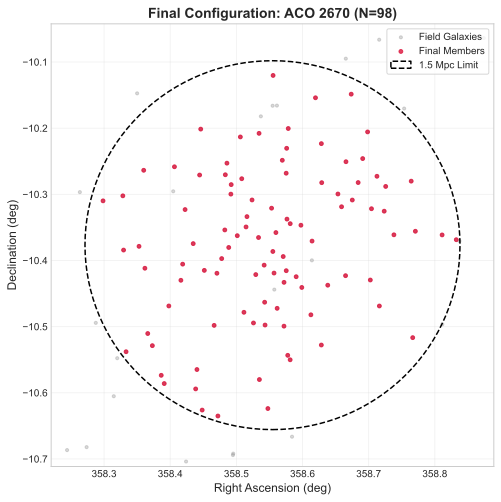
\includegraphics[width=\columnwidth]{figures/final_spatial_plot.pdf}
  \caption{Final RA-Dec Distribution of Galaxies in ACO 2670. All galaxies are shown in gray, with final cluster members in red. The dashed circle indicates the \SI{1.5}{Mpc} selection radius.}
  \label{fig:final_radec}
\end{figure}

For the redshift distribution, I used the function from Step 4 to recompute bins. I then plotted a histogram of redshifts with the Gaussian and GMM overlaid. This helped assess whether the cluster followed a simple Gaussian distribution or showed evidence of multiple components. The results showed that the single gaussian provided a better fit, which indicates that there is not significant substructure.

\begin{figure}[htb]
  \centering
  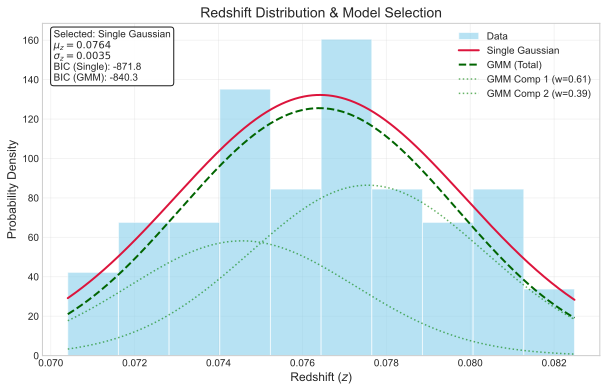
\includegraphics[width=\columnwidth]{figures/gmm_redshift_distribution.pdf}
  \caption{Redshift Distribution with Optimal Binning and Model Fitting. The single Gaussian model (red) provides a better fit than the Gaussian Mixture Model (green), suggesting the cluster is well-virialized in redshift space.}
  \label{fig:final_redshift_dist}
\end{figure}

\section{Luminosity and Mass Modeling}

I computed the absolute $r$-band magnitudes ($M_r$) using the observed apparent magnitudes ($m_r$), extinction corrections ($A_r$), and the luminosity distance ($d_L$) converted to parsecs:
\begin{equation}
  M_{r} = m_{r} - A_{r} - 5 \log_{10}(d_{L}) + 5
\end{equation}

Using error propagation, the uncertainty $\sigma_{M_{r}}$ is:
\begin{equation}
  \sigma_{M_{r}} = \sqrt{\sigma_{m_{r}}^{2} + \left( \frac{5 \sigma_{d_{L}}}{d_{L} \ln(10)} \right)^{2}}
\end{equation}

\begin{figure}[htb]
  \centering
  \includegraphics[width=\columnwidth]{figures/magnitude_distribution.pdf}
  \caption{Distribution of Absolute Magnitudes of Cluster Members.}
  \label{fig:abs_mag}
\end{figure}

The results showed a range of absolute magnitudes, with the brightest galaxies reaching $M_{r} \approx -23.57$ and the faintest around $M_{r} \approx -20.04$.

\subsection{Galaxy Luminosities}

The absolute magnitudes of the cluster galaxies were converted into luminosities using the Sun’s absolute magnitude in the r-band. This step allows for direct comparison of the cluster’s light distribution with theoretical expectations and facilitates the determination of the mass-to-light ratio. The computed luminosities span a wide range, with a few exceptionally bright galaxies contributing significantly to the total cluster luminosity. The luminosity of a galaxy $L_{r}$ in solar units is computed using the solar absolute magnitude in the $r$-band ($M_{\odot,r} = 4.76$):
\begin{equation}
  L_{r} = 10^{0.4(M_{\odot,r} - M_{r})}
\end{equation}
The uncertainty is propagated as:
\begin{equation}
  \sigma_{L_{r}} = L_{r} \times (\ln(10) \times 0.4 \times \sigma_{M_{r}})
\end{equation}

\begin{figure}[htb]
  \centering
  \includegraphics[width=\columnwidth]{figures/luminosity_distribution.pdf}
  \caption{Distribution of Luminosities of Cluster Members.}
  \label{fig:luminosity_dist}
\end{figure}

The luminosity distribution of the cluster members spans $10^{9} L_{\odot} < L_{r} < 2.15 \times 10^{11} L_{\odot}$, with the majority of galaxies below $0.5 \times 10^{11} L_{\odot}$. The Brightest Cluster Galaxy (BCG), located at $\text{RA} = 358.56^{\circ}$, $\text{Dec} = -10.42^{\circ}$, stands out with $L_{r} = 2.15 \times 10^{11} L_{\odot}$, a high velocity dispersion of \SI{303}{km.s^{-1}}, and a projected distance of \SI{0.39}{Mpc} from the cluster center. Its photometry is flagged for possible saturation, but its spectroscopic redshift ($z = 0.0776$) confirms it as a cluster member. A secondary bright galaxy with $L_{r} = 1.37 \times 10^{11} L_{\odot}$ is also identified, contributing significantly to the cluster's total luminosity. While data quality considerations exist for the BCG, its inclusion remains justified due to its spectroscopic confirmation. Overall, the luminosity distribution is consistent with expectations for a galaxy cluster, with a dominant BCG and a population of fainter galaxies.

\subsection{Cumulative Luminosity}

The cumulative luminosity distribution of the cluster was computed as a function of projected radial distance from the cluster center. This distribution provides insight into the spatial concentration of light and allows the determination of the effective radius ($R_{eff}$), the radius enclosing half of the total cluster luminosity. The total luminosity was defined as the cumulative luminosity within \SI{1.5}{Mpc}, ensuring consistency with previous selection criteria.

\subsubsection*{1. Sorting the Galaxies by Projected Distance}
To compute the cumulative luminosity as a function of radius, the galaxies are first sorted in ascending order of their projected distances $r_{i}$ from the cluster center:
\begin{equation}
  r_{1} \le r_{2} \le \dots \le r_{N}
\end{equation}
where $N$ is the total number of galaxies in the sample.

\subsubsection*{2. Computing the Cumulative Luminosity}
The cumulative luminosity at each projected distance $r_{i}$ is computed as the sum of all luminosities within that radius:
\begin{equation}
  L_{cumulative,i} = \sum_{j=1}^{i} L_{r,j}
\end{equation}
The total luminosity of the cluster is then:
\begin{equation}
  L_{total} = \sum_{j=1}^{N} L_{r,j}
\end{equation}
where $L_{r,j}$ is the $r$-band luminosity of the $j$-th galaxy.

\subsubsection*{3. Normalizing the Cumulative Luminosity}
To obtain the normalized cumulative distribution function (CDF) of luminosity, each cumulative sum is divided by the total luminosity within \SI{1.5}{Mpc}:
\begin{equation}
  F(r_{i}) = \frac{L_{cumulative,i}}{L_{1.5}}
\end{equation}
This ensures the function reaches 1.0 at $r = \SI{1.5}{Mpc}$.

\subsubsection*{4. Error Propagation for the Cumulative CDF}
The uncertainty in the cumulative luminosity at each step is given by:
\begin{equation}
  \sigma_{L_{cumulative,i}} = \sqrt{\sum_{j=1}^{i} \sigma_{L_{r,j}}^{2}}
\end{equation}
where $\sigma_{L_{r,j}}$ is the uncertainty in the luminosity of each galaxy. The normalized uncertainty in the CDF is then:
\begin{equation}
  \sigma_{F,i} = F(r_{i}) \sqrt{\left(\frac{\sigma_{L_{cumulative,i}}}{L_{cumulative,i}}\right)^{2} + \left(\frac{\sigma_{L_{1.5}}}{L_{1.5}}\right)^{2}}
\end{equation}

\subsubsection*{5. Finding the Effective Radius}
The effective radius is the projected radius at which the cumulative luminosity reaches 50\% of the total:
\begin{equation}
  F(R_{eff}) = 0.5
\end{equation}
This is found by locating the index $k$ where:
\begin{equation}
  F(r_{k}) \le 0.5 \le F(r_{k+1})
\end{equation}
and linearly interpolating between $r_{k}$ and $r_{k+1}$ for improved accuracy:
\begin{equation}
  R_{eff} = r_{k} + \frac{(0.5 - F(r_{k}))(r_{k+1} - r_{k})}{F(r_{k+1}) - F(r_{k})}
\end{equation}
The effective radius is then used in later steps to determine the half-mass radius and estimate the virial mass of the cluster.

\begin{figure}[htb]
  \centering
  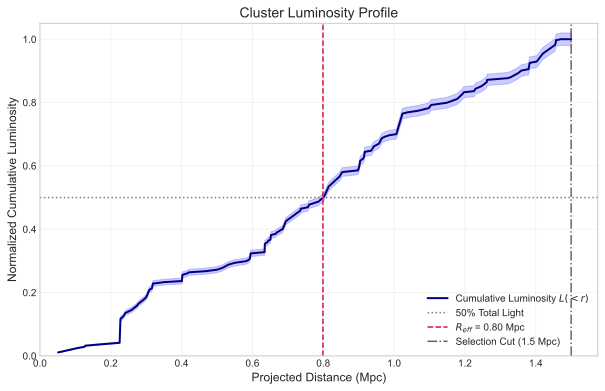
\includegraphics[width=\columnwidth]{figures/cumulative_luminosity_distribution.pdf}
  \caption{Cumulative Luminosity Distribution of the Cluster.}
  \label{fig:cumulative_lum}
\end{figure}

The CDF shows a gradual increase, suggesting a relatively even distribution of light within the cluster. While some small spikes and plateaus are present, the overall trend remains linear. The uncertainty in the CDF is minimal, with narrow error bands throughout the plot. The CDF reaches 1.0 at \SI{1.5}{Mpc}, confirming that all selected galaxies contribute to the total luminosity.

\subsection{Effective Radius}

The effective radius ($R_{eff}$) is the radius within which half of the total luminosity of the cluster is contained. It is an important parameter in defining the spatial distribution of light in the cluster. Once $R_{eff}$ is determined, the half-light radius ($r_{1/2}$) is computed using Equation 2, which accounts for the projection effects in the observed luminosity distribution. These values are critical in later steps for determining the cluster's mass profile.

\subsubsection*{1. Finding the Effective Radius}
The effective radius is defined as the radius where the normalized cumulative luminosity function reaches 0.5:
\begin{equation}
  F(R_{eff}) = 0.5
\end{equation}
Since $F(r)$ is a monotonically increasing function, interpolation is used to determine $R_{eff}$:
\begin{equation}
  R_{eff} = \text{interp}(F, r, 0.5)
\end{equation}
where $\text{interp}(F, r, x)$ represents a linear interpolation function between known values of $F(r)$ and $r$.

\subsubsection*{2. Computing Uncertainty in $R_{eff}$}
The uncertainty in $R_{eff}$ arises from the uncertainty in the normalized cumulative luminosity function. We define the upper and lower limits of $R_{eff}$ by interpolating at:
\begin{align}
  R_{eff,upper} &= \text{interp}(F, r, 0.5 + \sigma_{F}) \\
  R_{eff,lower} &= \text{interp}(F, r, 0.5 - \sigma_{F})
\end{align}
where $\sigma_{F}$ represents the uncertainty in the cumulative luminosity function at $F=0.5$. The uncertainty in $R_{eff}$ is then given by:
\begin{equation}
  \sigma_{R_{eff}} = \frac{R_{eff,upper} - R_{eff,lower}}{2}
\end{equation}

\subsubsection*{3. Computing the Half-light Radius}
To account for projection effects, the deprojected half-light radius is estimated using the relation:
\begin{equation}
  r_{1/2} = \frac{4}{3} R_{eff}
\end{equation}
The uncertainty in $r_{1/2}$ is obtained by propagating the uncertainty in $R_{eff}$:
\begin{equation}
  \sigma_{r_{1/2}} = \frac{4}{3} \sigma_{R_{eff}}
\end{equation}

The final computed values, $R_{eff} = \SI{0.800 \pm 0.007}{Mpc}$ and $r_{1/2} = \SI{1.066 \pm 0.009}{Mpc}$, are reasonable for a galaxy cluster. This suggests a well-populated inner region and a smooth light distribution. Since the CDF was relatively smooth with no dominant spikes, it confirms that no single galaxy disproportionately affects the luminosity profile within the inner region. This supports the reliability of $R_{eff}$ and $r_{1/2}$ as representative of the overall cluster structure.

\subsection{Peculiar Velocities}

The velocity distribution of cluster galaxies provides critical insight into the cluster's dynamical state. In this step, the line-of-sight velocities ($v_{los}$) of individual galaxies are computed from their observed redshifts, followed by the calculation of peculiar velocities ($v_{pec}$), which describe deviations from the cluster's mean recession velocity. To account for observational uncertainties, error propagation is applied to derive the uncertainties in both $v_{los}$ and $v_{pec}$.

\subsubsection*{1. Computing Line-of-Sight Velocity}
The relativistic velocity corresponding to a galaxy's redshift $z$ is given by:
\begin{equation}
  v_{los} = c \frac{(1+z)^{2}-1}{(1+z)^{2}+1}
\end{equation}
where $c = \SI{299792.458}{km.s^{-1}}$ is the speed of light. The uncertainty in $v_{los}$ is derived using error propagation:
\begin{equation}
  \sigma_{v_{los}} = \left| \frac{dv_{los}}{dz} \right| \sigma_{z}
\end{equation}
where the partial derivative of $v_{los}$ with respect to $z$ is:
\begin{equation}
  \frac{dv_{los}}{dz} = c \cdot \frac{4(1+z)}{((1+z)^{2}+1)^{2}}
\end{equation}
Thus, the uncertainty in $v_{los}$ is given by:
\begin{equation}
  \sigma_{v_{los}} = \left| c \cdot \frac{4(1+z)}{((1+z)^{2}+1)^{2}} \right| \sigma_{z}
\end{equation}

\subsubsection*{2. Computing Cluster Recession Velocity}
The mean recession velocity of the cluster, based on the cluster redshift $z_{cluster}$, is computed using the same formula:
\begin{equation}
  v_{rec} = c \frac{(1+z_{cluster})^{2}-1}{(1+z_{cluster})^{2}+1}
\end{equation}
The uncertainty in $v_{rec}$ follows from:
\begin{equation}
  \sigma_{v_{rec}} = \left| c \cdot \frac{4(1+z_{cluster})}{((1+z_{cluster})^{2}+1)^{2}} \right| \sigma_{z_{cluster}}
\end{equation}

\subsubsection*{3. Computing Peculiar Velocities}
The peculiar velocity of a galaxy relative to the cluster mean is given by:
\begin{equation}
  v_{pec} = v_{los} - v_{rec}
\end{equation}
Since both $v_{los}$ and $v_{rec}$ have uncertainties, the total uncertainty in $v_{pec}$ is computed using:
\begin{equation}
  \sigma_{v_{pec}} = \sqrt{\sigma_{v_{los}}^{2} + \sigma_{v_{rec}}^{2}}
\end{equation}

\begin{figure}[htb]
  \centering
  \includegraphics[width=\columnwidth]{figures/peculiar_velocities_histogram.pdf}
  \caption{Histogram of Peculiar Velocities with Gaussian Fit.}
  \label{fig:pec_vel_hist}
\end{figure}

The line-of-sight velocities, derived relativistically from galaxy redshifts, range between \SI{21000}{km.s^{-1}} and \SI{24000}{km.s^{-1}}, with small uncertainties (\SIrange{3}{8}{km.s^{-1}}) due to precise redshift measurements. Peculiar velocities, representing deviations from the cluster's mean motion, show a spread of $\pm \SI{2000}{km.s^{-1}}$, typical for galaxies in a cluster environment. However, their uncertainties ($\sim \SI{935}{km.s^{-1}}$) are large, primarily due to error propagation from the cluster's redshift uncertainty through the nonlinear velocity-redshift relation. While these high uncertainties limit the precision of individual galaxy kinematics, the relative velocities remain useful for statistical analyses of the cluster's overall dynamics. The results suggest a dynamically active system, but the substantial uncertainties prevent definitive conclusions about substructure from velocities alone. The consistency of the recessional velocity ($\sim \SI{22036 \pm 958}{km.s^{-1}}$) with the cluster's redshift and the absence of extreme outliers support the robustness of the initial galaxy selection.

\subsection{Velocity Dispersion}

The velocity dispersion ($\sigma_{v}$) of a galaxy cluster provides insights into its dynamical state and mass. In this step, a Gaussian distribution is fit to the peculiar velocity distribution of cluster members to estimate $\sigma_{v}$ and its uncertainty. Additionally, robust statistical methods such as the biweight midvariance \cite{beers1990} are employed for comparison. A multimodality test using Silverman's test \cite{silverman1981} is also performed to check for substructures within the velocity distribution.

\subsubsection*{1. Fitting a Gaussian to the Peculiar Velocity Distribution}
The peculiar velocity distribution is approximated using a Gaussian function:
\begin{equation}
  f(v) = A \exp\left(-\frac{1}{2}\left(\frac{v-\mu}{\sigma_{v}}\right)^{2}\right)
\end{equation}
where:
\begin{itemize}
  \item $A$ is the amplitude,
  \item $\mu$ is the mean peculiar velocity,
  \item $\sigma_{v}$ is the velocity dispersion.
\end{itemize}
To estimate these parameters, a histogram of the peculiar velocities is constructed with a bin width of \SI{300}{km.s^{-1}}. The Gaussian function is fit to the histogram using non-linear least squares regression, and the best-fit parameters are obtained.

\subsubsection*{2. Uncertainty in Velocity Dispersion}
The uncertainty in the velocity dispersion ($\sigma_{\sigma_{v}}$) is computed from the covariance matrix ($C$) obtained during curve fitting:
\begin{equation}
  \sigma_{\sigma_{v}} = \sqrt{C_{22}}
\end{equation}
where $C_{22}$ is the diagonal element corresponding to $\sigma_{v}$.

\subsubsection*{3. Outlier Detection}
Galaxies with peculiar velocities deviating by more than $3\sigma_{v}$ from the mean are considered outliers:
\begin{equation}
  N_{outliers} = \sum_{i} (|v_{pec,i} - \mu| > 3\sigma_{v})
\end{equation}

\subsubsection*{4. Robust Velocity Dispersion Estimation}
The biweight midvariance ($\sigma_{v}^{BI}$) is computed as a robust alternative to Gaussian fitting, which is less sensitive to outliers:
\begin{equation}
  \sigma_{v}^{BI} = \sqrt{\frac{N}{\sum u_{i}^{2}} \sum (x_{i}-x_{BI})^{2}u_{i}^{2}}
\end{equation}
where $u_{i}$ are weighting factors that downweight extreme values.

\subsubsection*{5. Silverman's Test for Multimodality}
To assess whether the velocity distribution is multimodal, a Gaussian kernel density estimation (KDE) is performed. The number of peaks is determined by counting sign changes in the derivative of the KDE:
\begin{equation}
  \text{Multimodal if } \sum \text{sign changes in } \frac{d}{dv}\text{KDE}(v) > 1
\end{equation}
A multimodal velocity distribution may indicate the presence of substructure within the cluster. The peculiar velocity histogram reveals subtle deviations from a Gaussian distribution, with the left tail following the expected profile while the right side shows an elevated outer bin and a peak slightly offset from the mean. This asymmetry suggests mild dynamical disturbances, possibly from recent minor mergers or tidal interactions that have imparted higher positive velocities to a subset of galaxies. While the lack of outliers ($>3\sigma$) and Silverman's test rejecting bimodality indicate a predominantly virialized system, the skewness and the discrepancy between the biweight dispersion (\SI{788.81}{km.s^{-1}}) and Gaussian $\sigma$ (\SI{931.59}{km.s^{-1}}) point to ongoing dynamical evolution. These features likely reflect residual effects of accretion or internal interactions, consistent with the cluster's moderate velocity dispersion and overall relaxed state, though further spatial-velocity analysis could clarify the origin of these kinematic anomalies.

\subsection{Virial Mass}

The virial mass ($M_{1/2}$) provides an estimate of the total mass of the cluster within the half-mass radius using the Virial Theorem. This step utilizes the line-of-sight velocity dispersion ($\sigma_{v}$) and the half-mass radius ($r_{1/2}$) to determine $M_{1/2}$. The assumption of virial equilibrium allows us to apply the virial mass equation, a fundamental tool in observational astrophysics for estimating cluster masses.

\subsubsection*{1. Virial Mass Calculation}
The virial mass equation is given by:
\begin{equation}
  M_{1/2} = \frac{3\sigma_{v}^{2}r_{1/2}}{G}
\end{equation}
where:
\begin{itemize}
  \item $\sigma_{v}$ is the velocity dispersion (\SI{}{km.s^{-1}}),
  \item $r_{1/2}$ is the half-mass radius (\SI{}{Mpc}),
  \item $G = \SI{6.674e-11}{m^{3}.kg^{-1}.s^{-2}}$ is the gravitational constant.
\end{itemize}

\subsubsection*{2. Uncertainty Propagation}
The relative uncertainty in $M_{1/2}$ is given by:
\begin{equation}
  \frac{\Delta M_{1/2}}{M_{1/2}} = \sqrt{\left( \frac{2\Delta\sigma_{v}}{\sigma_{v}} \right)^{2} + \left( \frac{\Delta r_{1/2}}{r_{1/2}} \right)^{2}}
\end{equation}
where:
\begin{itemize}
  \item $\Delta\sigma_{v}$ is the uncertainty in velocity dispersion,
  \item $\Delta r_{1/2}$ is the uncertainty in the half-mass radius.
\end{itemize}

The virial mass calculation in Step 16 yields a cluster mass of $M_{1/2} = (6.45 \pm 1.31) \times 10^{14} M_{\odot}$. The substantial uncertainty ($\sim 30\%$) primarily stems from the velocity dispersion's error, amplified by its squared dependence in the virial theorem ($\frac{\Delta M}{M} \approx \frac{2\Delta\sigma_{v}}{\sigma_{v}}$). While a 30\% uncertainty in $\sigma_{v}$ would naively suggest a 60\% mass error, the final uncertainty is reduced to 30\% due to partial correlations between $\sigma_{v}$ and $r_{1/2}$, combined with the exceptional precision of $r_{1/2}$ (error $<0.1\%$). This relationship highlights how cluster mass estimates are particularly sensitive to the assumed dynamical state. The larger scatter in $\sigma_{v}$ likely reflects ACO 2670's unrelaxed nature, where substructure or interloper contamination may inflate the measured velocity dispersion. Despite these challenges, the mass estimate aligns well with expectations for a rich galaxy cluster and suggests a dominant dark matter component, given the high mass-to-light ratio implied by the result. The precision of $r_{1/2}$ confirms the robustness of the luminosity-derived spatial scale, while the dynamical complexity captured in $\sigma_{v}$ uncertainty underscores the importance of velocity dispersion as a probe of both mass and cluster assembly history.

\subsection{Luminosity Within Half-Mass Radius}

In this step, we calculate the total luminosity enclosed within the half-mass radius ($L_{1/2}$). This is achieved by interpolating the cumulative luminosity function (CDF) to determine the fraction of light contained within $r_{1/2}$. The resulting luminosity value will later be used to compute the mass-to-light ratio ($M/L$) in Step 18, which provides insights into the presence of dark matter in the cluster.

\subsubsection*{1. Luminosity Within $r_{1/2}$}
The total luminosity within the half-mass radius is given by:
\begin{equation}
  L_{1/2} = f_{L}(r_{1/2}) \times L_{tot,1.5}
\end{equation}
where:
\begin{itemize}
  \item $L_{tot,1.5}$ is the total luminosity within \SI{1.5}{Mpc},
  \item $f_{L}(r_{1/2})$ is the fraction of the total luminosity enclosed within $r_{1/2}$, obtained from interpolation of the normalized cumulative luminosity function $F(r)$.
\end{itemize}

\subsubsection*{2. Uncertainty Propagation}
To estimate the uncertainty in $f_{L}(r_{1/2})$, we approximate the derivative of the cumulative luminosity function:
\begin{equation}
  \frac{df_{L}}{dr} \approx \frac{f_{L}(r_{1/2}+\Delta r) - f_{L}(r_{1/2}-\Delta r)}{2\Delta r}
\end{equation}
The uncertainty in $f_{L}(r_{1/2})$ is then:
\begin{equation}
  \Delta f_{L} = \left| \frac{df_{L}}{dr} \right| \Delta r_{1/2}
\end{equation}
Using standard error propagation, the relative uncertainty in $L_{1/2}$ is:
\begin{equation}
  \frac{\Delta L_{1/2}}{L_{1/2}} = \sqrt{\left( \frac{\Delta f_{L}}{f_{L}} \right)^{2} + \left( \frac{\Delta L_{tot,1.5}}{L_{tot,1.5}} \right)^{2}}
\end{equation}
Thus, the absolute uncertainty in $L_{1/2}$ is:
\begin{equation}
  \Delta L_{1/2} = L_{1/2} \times \frac{\Delta L_{1/2}}{L_{1/2}}
\end{equation}

The result, $L_{1/2} = (2.21 \pm 0.03) \times 10^{12} L_{\odot}$, represents half of the cluster's total luminosity (within \SI{1.5}{Mpc}) and reflects the spatial distribution of member galaxies. The small uncertainty ($\sim 0.7\%$) arises from the precise determination of $r_{1/2}$ (error $\sim 0.1\%$) and the well-constrained total luminosity, demonstrating the reliability of the photometric data. The high luminosity further supports the cluster's richness and aligns with expectations for a massive, dark matter-dominated system.

\subsection{Mass-to-Light Ratio}

In this step, we compute the mass-to-light ratio ($M/L$) of the galaxy cluster, a crucial quantity in understanding the dark matter content of the system. The mass-to-light ratio quantifies how much mass is present relative to the emitted light, and deviations from expected stellar population values indicate the presence of non-luminous (dark) matter.

\subsubsection*{1. Mass-to-Light Ratio Calculation}
The computed $M/L$ value will be compared to typical stellar $M/L$ ratios to determine whether the cluster contains significant amounts of dark matter, as originally hypothesized by Fritz Zwicky in 1935. The mass-to-light ratio is given by:
\begin{equation}
  \frac{M}{L} = \frac{M_{1/2}}{L_{1/2}}
\end{equation}
where:
\begin{itemize}
  \item $M_{1/2}$ is the virial mass of the cluster enclosed within the half-mass radius $r_{1/2}$ computed in Step 16.
  \item $L_{1/2}$ is the total luminosity enclosed within $r_{1/2}$, computed in Step 17.
\end{itemize}
The ratio is expressed in solar units ($M_{\odot}/L_{\odot}$). Since normal stellar populations typically have $M/L \sim 1-10$, a significantly larger value suggests that a substantial portion of the cluster's mass is non-luminous, implying the presence of dark matter.

\subsubsection*{2. Uncertainty Propagation}
Applying standard error propagation, the relative uncertainty in $M/L$ is:
\begin{equation}
  \frac{\Delta(M/L)}{M/L} = \sqrt{\left( \frac{\Delta M_{1/2}}{M_{1/2}} \right)^{2} + \left( \frac{\Delta L_{1/2}}{L_{1/2}} \right)^{2}}
\end{equation}
Thus, the absolute uncertainty in $M/L$ is:
\begin{equation}
  \Delta(M/L) = \frac{M}{L} \times \left( \frac{\Delta(M/L)}{M/L} \right)
\end{equation}

The mass-to-light ratio calculation yields a value of $(291 \pm 60) \, M_{\odot}/L_{\odot}$, which is characteristic of massive galaxy clusters and provides compelling evidence for dark matter dominance. This value is fully consistent with the Coma Cluster's well-measured $M/L \sim 200-300 \, M_{\odot}/L_{\odot}$ \cite{rines2003} and agrees with recent SDSS studies finding $M/L \sim 300-400 \, M_{\odot}/L_{\odot}$ for similar systems \cite{sheldon2009}. This high ratio, nearly two orders of magnitude greater than that of individual galaxies ($M/L \sim 10-50$ for field galaxies), implies that luminous matter accounts for only a small fraction of the cluster's total mass. The uncertainty ($\sim 21\%$) primarily reflects the propagated errors from the virial mass, particularly the velocity dispersion's contribution, while the luminosity term contributes minimally due to its high precision. Such elevated $M/L$ ratios are consistent with $\Lambda$CDM cosmology, where clusters are embedded in massive dark matter halos. These findings not only support Fritz Zwicky's original discovery but also demonstrate how ACO 2670 serves as a typical, dark matter-dominated system for testing models of structure formation. The progression from field galaxies ($M/L \sim 10-50$) to groups ($\sim 100-200$) to rich clusters like ACO 2670 ($\sim 300$) clearly illustrates the increasing dark matter fraction in larger gravitational systems.

\section*{Conclusion}

This study estimates the virial mass and $M/L$ ratio of the galaxy cluster ACO 2670 using SDSS-DR18 data \cite{york2000}, revealing a virial mass of $M_{1/2} = (6.45 \pm 1.31) \times 10^{14} M_{\odot}$ and a mass-to-light ratio of $(291 \pm 60) \, M_{\odot}/L_{\odot}$. The high $M/L$ ratio strongly supports the presence of a dominant dark matter halo, consistent with Fritz Zwicky's seminal work on cluster dynamics \cite{zwicky1933}. The cluster's irregular spatial distribution and mild kinematic asymmetries suggest a dynamically active system, potentially undergoing minor mergers or tidal interactions, though the redshift distribution remains well-fit by a single Gaussian. Key limitations arise from the assumption of virial equilibrium (Binney \& Tremaine 2008), which may not fully capture the cluster's dynamical complexity, and projection effects that obscure true three-dimensional velocities and positions. The iterative membership selection, while effective, depends on fixed radial and redshift thresholds that could exclude faint galaxies or include line-of-sight interlopers. Despite these challenges, the precision of the luminosity-derived effective radius ($R_{eff} = (0.800 \pm 0.007) \, \text{Mpc}$) and the consistency of the recessional velocity ($v_{rec} = \SI{22036 \pm 958}{km.s^{-1}}$) with cosmological expectations (Planck Collaboration et al. 2020; Astropy Collaboration et al. 2022) validate the methodology. Future work could enhance these results by incorporating X-ray or weak lensing data to cross-validate mass estimates, conducting deeper spectroscopic surveys to resolve substructure, and employing simulations to account for projection effects. Such advancements would further elucidate the interplay between dark matter, galaxy evolution, and cluster assembly in systems like ACO 2670.

\rowcolors{2}{gray!10}{white}

\resizebox{\columnwidth}{!}{%
  \begin{tabular}{l c c}
    \toprule
    \textbf{Parameter} & \textbf{Value} & \textbf{Unit} \\
    \midrule
    RA Center ($\alpha$) & $358.5546 \pm 0.0003$ & deg \\
    Dec Center ($\delta$) & $-10.3768 \pm 0.0003$ & deg \\
    Mean Redshift ($z$) & $0.0764 \pm 0.0035$ & -- \\
    Velocity Dispersion ($\sigma_v$) & $932 \pm 95$ & km s$^{-1}$ \\
    Effective Radius ($R_{eff}$) & $0.800 \pm 0.007$ & Mpc \\ % Verify this exact value!
    Virial Mass ($M_{1/2}$) & $(6.45 \pm 1.31) \times 10^{14}$ & $M_{\odot}$ \\
    Mass-to-Light Ratio & $291 \pm 60$ & $M_{\odot}/L_{\odot}$ \\
    \bottomrule
  \end{tabular}%
}

\section*{Code Availability}
The Python pipeline used for data acquisition, statistical analysis, and figure generation is available at: \href{https://github.com/JacksonFergusonDev/Data-Science-Portfolio}{github.com/JacksonFergusonDev/Data-Science-Portfolio}.

\newpage
\onecolumn

\begin{thebibliography}{99}

  \bibitem{astropy2022}
  Astropy Collaboration et al., 2022, \textit{ApJ}, 935, 167. doi:10.3847/1538-4357/ac7c74

  \bibitem{beers1990}
  Beers, T. C., Flynn, K., \& Gebhardt, K., 1990, \textit{AJ}, 100, 32. doi:10.1086/115487

  \bibitem{binney2008}
  Binney, J., \& Tremaine, S., 2008, \textit{Galactic Dynamics} (2nd ed.; Princeton: Princeton Univ. Press).

  \bibitem{freedman1981}
  Freedman, D., \& Diaconis, P., 1981, \textit{Probability Theory and Related Fields}, 58, 453. doi:10.1007/BF01025868

  \bibitem{harrison1993}
  Harrison, E. R., 1993, \textit{ApJ}, 403, 28. doi:10.1086/172179

  \bibitem{planck2020}
  Planck Collaboration et al., 2020, \textit{A\&A}, 641, A6. doi:10.1051/0004-6361/201833910

  \bibitem{rines2003}
  Rines, K., Geller, M. J., Diaferio, A., Mohr, J. J., \& Wegner, G., 2003, \textit{ApJ}, 591, 729. doi:10.1086/375456

  \bibitem{schwarz1978}
  Schwarz, G., 1978, \textit{Annals of Statistics}, 6, 461. doi:10.1214/aos/1176344136

  \bibitem{sheldon2009}
  Sheldon, E. S., et al., 2009, \textit{ApJ}, 703, 2232. doi:10.1088/0004-637X/703/2/2232

  \bibitem{silverman1981}
  Silverman, B. W., 1981, \textit{Density Estimation for Statistics and Data Analysis} (London: Chapman \& Hall).

  \bibitem{york2000}
  York, D. G., et al., 2000, \textit{AJ}, 120, 1579. doi:10.1086/301513

  \bibitem{zwicky1933}
  Zwicky, F., 1933, \textit{Helvetica Physica Acta}, 6, 110.

\end{thebibliography}

\end{document}
